\documentclass{article}
\usepackage[utf8]{inputenc}
\usepackage{graphicx}
\graphicspath{ {./images/} }
\usepackage{amsmath}
\usepackage{hyperref}
%\usepackage[english]{babel}
\usepackage{longtable}
\usepackage[left=2cm,right=1cm, top=2cm,bottom=2cm,bindingoffset=0cm]{geometry}

\renewcommand{\normalsize}{\fontsize{14}{18pt}\selectfont}
\newcommand{\specialcell}[2][c]{%
	\begin{tabular}[#1]{@{}c@{}}#2\end{tabular}}
\title{ Gene prediction for mystery Tardigrades genomes }
\author{ Ignat Sonets, Kamilla Faizullina}
\date{\empty}

\begin{document}
	\catcode`\_=\active
\maketitle
 
 
 In this report we try to find new proteins somehow related to DNA repair mechanisms of tardigrades. As a model Ramazzottius varieornatus, the YOKOZUNA-1 strain was selected, and genome annotation data and mass spectrometry results were obtained. After analysis made, we found at least 2 candidate proteins which have  nuclear localization, DNA-binding activity,as also they participate in recombination and mechanisms. Our results can partially explain the survivability of tardigrades in various harsh conditions.
 
 
\section{Introduction}
 
 Greetings! Today we present you our results about searching DNA repair mechanisms in tardigrades. But before we start, let's do a quick walkthrough about Tardigrades itself and methods used in this project.
 Tardigrades, also known as as water bears or moss piglets, are a phylum of eight-legged segmented micro-animals. They were first described by the German zoologist Johann August Ephraim Goeze in 1773, who called them little water bears. In 1777, the Italian biologist Lazzaro Spallanzani named them Tardigrada, which means "slow steppers"\cite{1}. 
 They have 2 distinct traits:
 
 1. They are almost indestructible. They could have been found everywhere, literally everywhere: in Earth's biosphere, from mountaintops to the deep sea and mud volcanoes, and from tropical rainforests to the Antarctic \cite{1}. Tardigrades are among the most resilient animals ever known to man. They have anomalous endurance in terms of survivability of extreme conditions, and even deep dead space filled with vacuum and radiation emitted from myriads of stars could nothing to do. They are truly space marines coming from the Earth. They exist ca. 500 million years and I guess will exist for nest 500 million years. They are living grey goo in size of approx. 0.5 mm, thousands of little Thanoses. But what makes them so adapted to everything? First, they developed  anhydrobiosis, cryobiosis, osmobiosis, or anoxybiosis, and so on. Depending on the environment, they simply go to sleep forming capsule around ther bodies,thus preserving resources and waiting for shiny weather. Second (and it would be our task) they seem to have some mechanisms providing DNA repair to escape the death and different pathologies. They m u s t definitely have a galore of these methods. Let's find them! But before we start, the second trait:
 
 2. They are extremely cute. %$^_^$
 
 So, what about the data we have? We will be using the sequence of the Ramazzottius varieornatus, the YOKOZUNA-1 strain, its annotation provided by our team, and mass spectrometry data of chromatin of this water bear. The core idea in this project is that tardigrades might have unique proteins associated with their DNA to protect and/or effectively repair it. To put in simple, we will merge proteome data and genome data, and try to find any intersections, determine physical localization of found proteins, and try to explain and discuss our findings.
 
 Also we need to briefly mention different tools we used. 
 AUGUSTUS tool is a gene prediction tool running a generalized hidden Markov model (GHMM), which defines probability distributions for the various sections of genomic sequences. Introns, exons, intergenic regions, etc. correspond to states in the model and each state is thought to create DNA sequences with certain pre-defined emission probabilities. Similar to other HMM-based gene finders, AUGUSTUS finds an optimal parse of a given genomic sequence, i.e. a segmentation of the sequences into states that is most likely according to the underlying statistical model. 
 
 BLAST is a gold standard alignment tool that searches for homology (i.e. similarity between sequences.For more info, please view \cite{4}.) between query sequence and desired database containing pre-analysed data. BLAST identifies homologous sequences using a heuristic method which initially finds short matches between two sequences; thus, the method does not take the entire sequence space into account. After initial match, BLAST attempts to start local alignments from these initial matches. This also means that BLAST does not guarantee the optimal alignment, thus some sequence hits may be missed. In order to find optimal alignments, the Smith-Waterman algorithm should be used \cite{2, 3}.
  
 Brief introduction about other used tools are given in Task4 document.
 
 
 \section{Data}
 We use the assembled genome data of the Ramazzottius varieornatus, the YOKOZUNA-1 strain \cite{data}. 
 
 
 
 

\section{Methods}
 We use the implemented program AUGUSTUS for gene prediction \cite{augustus}. This program is specified for eukaryotic sequencing data. Usually the number of obtained proteins is too large. 
 
 In order to detect regions, linked to DNA repair, we should use both genomic and proteomic data. We can use a list of peptides that were associated with the DNA regions. This list can be obtained via analyzis of extracted chromatin fraction using tandem mass spectrometry. To find associated proteins from the R. varieornatus genome  to peptides, we use $\textrm{makeblastdb}$ utilite \cite{blast}.
 
 Net, to narrow the list of proteins, we use WoLF PSORT \cite{WOlf}. This program allows to predict where these proteins are found in the cell based on their sequences. predicts the subcellular localization of proteins. The method is based on detection the presence of a signal peptide on their N-terminus. We also use TargetP 1.1 Server \cite{ptarget}, which also predicts the subcellular localization.
 
 To find homologous proteins we use Blast \cite{2}. We use HMMER to predict the function of the proteins \cite{HMM}. The HMMER is based on Hidden Markov Models.  
 

\section{Results}
 \begin{figure}[h]
 	\centering
 	\includegraphics[scale=0.63]{tree}  
 	\caption{ Fylogenetic tree.}
 	\label{tree}
 \end{figure}
  First, our goal is to make functional annotation. So, we run AUGUSTUS to find homologous proteins in tardigrade genome data. We used training sets  Acyrthosiphon pisum species via augustus. We have chosen this species after  fylogenetic tree construction \ref{tree}.   We obtained $14446$ proteins. 
 
 Next, we used the list of peptides and command \emph{makeblastdb}. After removing duplicates, we got 31 proteins. After using Blast alignment, we keeped 22 proteins. The summury information is presented in Table \ref*{tab:rarevars}.
 \begin{longtable}[H!]{|c|c|c|c|c|c|c|} 
 	%{||c c c c c c c||}
 	%\centering
 	%\begin{tabular}{|c|c|c|c|c|c|c|}
  	\hline
 		id & cover &  	E-value	&  Identity & WolF & TargetP &	HMMER \\
 		 		\hline
 		g5214t1 & 32  &	1e-12 & 39.29 & \specialcell{*nucl: 4.5, \\ cytonucl: 5.5}  & Other & \specialcell{ Chitin binding \\Peritrophin-A \\ domain}  \\ 
	\hline
  		g11539t1 & 50  &	3e-06 & 28.57 & \specialcell{ }  & \specialcell{Signal \\ peptide} & \specialcell{  }  \\ 
 \hline
  		g5192t1 & 40  &		2e-14 & 40 & \specialcell{ }  & \specialcell{Signal \\ peptide} & \specialcell{Chitin binding \\
  			Peritrophin-A
  			\\ domain}  \\ 
 \hline
  		g5086t1 & 12  &	2e-6 & 44& \specialcell{ }  &   \specialcell{Signal \\ peptide}  & \specialcell{ Chitin binding \\Peritrophin-A \\ domain}  \\ 
 \hline
  		g5087t1 & 20  &	6e-13 & 40 & \specialcell{nucl: 9}  & Other & \specialcell{ Chitin binding \\Peritrophin-A \\ domain}  \\ 
 \hline
  		g672t1 & 28  &	1e-5 & 42 & \specialcell{ }  &  \specialcell{Signal \\ peptide}  & \specialcell{ Chitin binding \\Peritrophin-A \\ domain}  \\ 
 \hline
  		g7315t1 & 96  &	8e-70 & 38  & \specialcell{nucl: 17.5, \\ cytonucl: 15.5 }  & Other & \specialcell{ SNF2 family \\
  			N-terminal \\  
  			domain}  \\ 
 \hline
 
   		g2692t1 & 12  &	1e-3 & 26  & \specialcell{*cytonucl: 4, \\  nucl: 3.5}  & Other & \specialcell{ Hermes \\ 
   			transposase \\ 
   			DNA-binding \\ 
   			domain}  \\ 
 \hline
 	
   		g4653t1 & 54 &	1e-13 & 36  & \specialcell{ }  & Other & \specialcell{Zinc finger }  \\ 
\hline

 
 
   		g8025t1 & 48   &	8e-104 & 38  & \specialcell{  }  & Other & \specialcell{ Cytosol \\
   			amino
   			\\ peptidase \\
   			family, \\ catalytic \\
   			domain}  \\ 
 \hline
 
   		g3168t1 & 97   &	8e-50 & 48  & \specialcell{   }  & Other & \specialcell{ }  \\ 
 \hline
 
   		g10626t1 & 72  &	8e-82 & 27  & \specialcell{  }  & Other & \specialcell{ Transport \\ 
   			protein Trs120 \\ 
   			or TRAPPC9, \\
   			TRAPP II \\ 
   			complex \\ 
   			subunit}  \\ 
 \hline

    		g1221t1 & 13  &	1e-20 & 43  & \specialcell{  }  &  \specialcell{Signal \\ peptide}  & \specialcell{ Casein \\ kinase \\
    			substrate \\ 
    			phosphoprotein \\ 
    			PP28}  \\ 
 \hline
 
    		g10444t1 & 9  &	3e-3 & 27  & \specialcell{ }  &  \specialcell{Signal \\ peptide} & \specialcell{  }  \\ 
 \hline
 
 
    		g7708t1 & 93  &	2e-35 & 22  & \specialcell{ nucl: 15.5,\\ cytonucl: 15.5 }  & Other & \specialcell{ Region in \\
    			Clathrin and \\
    			VPS}  \\ 
 \hline
  
  
  
  
      		g5481 & 13  &	1e-11 & 35  & \specialcell{  nucl: 27, \\  cytonucl: 18.3333}  & Other & \specialcell{  }  \\ 
  \hline
  
      		g7708t1 & 93  &	2e-35 & 22  & \specialcell{ nucl: 15.5,\\ cytonucl: 15.5  }  & Other & \specialcell{ Region in \\
  	Clathrin and \\
  	VPS}  \\ 
  \hline
  
  
      		g7784t1 & 83  &	2e-90 & 36  & \specialcell{ nucl: 9.5 \\ cytonucl: 6 }  &  \specialcell{Signal \\ peptide}  & \specialcell{ Glycosyl \\
      			transferase \\
      			family 2}  \\ 
  \hline
  
  
      		g11028t1 & 98  &	2e-82 & 26  & \specialcell{ nucl: 32,\\   }  & Other & \specialcell{ Zinc finger,\\
      			C3HC4 type \\
      			(RING finger)}  \\ 
  \hline
  
  
  
      		g3380t1 & 51  &	4e-8 & 24  & \specialcell{
      		
      	*cytonucl: 1.83333, \\ nucl: 1.5 
       }  &  \specialcell{Signal \\ peptide}   & \specialcell{ Astacin \\ 
       (Peptidase \\ 
       family M12A)}  \\ 
  \hline
  
  
  
      		g9785t1 & 29  &	1e-5 & 33  & \specialcell{ nucl: 16 }  & Other & \specialcell{ }  \\ 
  \hline
  
  
  
    
  g2090t1 & 73  &	2e-126 & 36  & \specialcell{*nucl: 2\\  }  & Other & \specialcell{ Glycosyl \\
  	hydrolases \\
  	family 31}  \\ 
  \hline
 
 		
 		\hline
\caption[LOF entry]{Summary information. The star in cell WolF (localization) means that nucl and cytonucl are not maximum. The empty cell means that information is not presented.}
 	\label{tab:rarevars}
 \end{longtable}
 
 
 
\section{Discussion}
 So, we run AUGUSTUS to find homologous proteins in tardigrade genome data. To detect conserved domains, we used training sets Acyrthosiphon pisum species via AUGUSTUS. We obtained 14446 proteins. After creating local BLAST database and doing a BLAST, we obtained 31 unique hits, which were used in downstream analysis.
 
 Using multiple tools, we successfully combined results from various sources, thus allowing to find only desired proteins: Selection criteria were:
 
 1. WoLFPROT: predominantly localisation in nucleus/cytonucleus(the bigger score, the better its confidence in localisation in one compartment)
 
 2. hmmscan: desired top hits (with minimum of E-value). Although useful in common sense, here we're not interested in carbohydrates metabolism or Golgi complex proteins.
 
 3. TargetP: not signal proteins, because we need proteins that are constantly present in cell nucleus to maintain chromatin stability.
 4. BLAST: max score/% of identity, but minimal E-value, and proteins corresponding our goal.
 
 All the data are in Table \ref{tab:rarevars}.
 
 According to these criteria, at least 2 proteins passed this filtration. First we present the top hits for each protein. There are g7315_t1, which is SNF2 family N-terminal domain(Pfam PF00176.23) and HepA-related protein (HARP)(Pfam PF07443.13), and g11028\_t1(Zinc finger, C3HC4 type (RING finger)(Pfam PF00097.25)). 1 more protein, g4563_t1, could be potentially interpreted as Zinc knuckle(Pfam PF00098.23), although it's not the best hit for this protein. Fig.2,3,4 provides more detailed data about best hits. BLAST against SwissProt/UniProt database partially confirms our results. For g7315_t1, best BLAST hit is HepA-related protein(Uniprot B4F769) for g11028_t1, best BLAST hit is RING-type E3 ubiquitin transferase rad18(Uniprot Q4WZJ6).
 
 According to the article provided with Task, we found neither MRE11 protein, nor Dsup protein, which is confusing. Perhaps if we use pre-computed AUGUSTUS annotation, we will find them. Although we didn't find specific proteins related to tardigrades 'genetic endurance', we still found proteins related to DNA repair and chromosome maintenance. Thinking that only 2 genes wiil do all the magic is naive and suitable only for newcomers in biology, so I think we reached a partial, but success. To better explain this, I would like to provide some description for each protein we found. For other details please use provided Pfam codes. Thanks to tight integration with Uniprot database, you can easily access additional info! WARNING! Some parts of the text below are taken without changes from its Pfam/UniProt articles. It's not a plagiarism--I just can't write it better than it is. 
 To be honest, not all of our findings are proteins. Some of them are just their domains, like our first hero--SNF2 family N-terminal domain. As far as I know, one protein domain performs 1 specific function. SNP NTD domain is a part of proteins which involved in many functions transcription regulation, DNA repair (The most important for us!This domain is a part pf e.g. ERCC6, protein that conduct excision repair. This protein has ATPase activity thanks to this domain. Damaging this domain could ruin functioning of ERCC6 as the whole. More info about ERCC6 here \cite{5}), DNA recombination and chromatin unwinding.
 Our second candidate for g7315 is a protein--HepA-related protein, also known as SMARCAL1 (SWI/SNF-related, matrix-associated, actin-dependent regulator of chromatin, subfamily A-like1), also known as DNA-dependent ATPase A. Its function is maintaining genome integrity during DNA replication, working as helicase and stabilisng replication forks in right orientation. The last candidate for g7315_t1...it's not much to say. Presumably it's Type III restriction enzyme, res subunit, and that's all. Without exact knowing of which is this restrictase we can only assume its(g7351) participation in DNA-related activity, such as participation in recombination. And we are wery glad that BLAST confirms this protein too!
 
 For g11028 we did find only domain, so we can only speculate about which specific protein this domain belongs. A RING (Really Interesting New Gene) finger domain is a protein domain of zinc finger type which contains a C3HC4 amino acid motif which binds two zinc cations (seven cysteines and one histidine arranged non-consecutively).This protein domain contains from 40 to 60 amino acids. Many proteins containing a RING finger play a key role in the ubiquitination pathway \cite{6}. Whatever the exact protein is, we know its fuctions--ubiquitination and/or DNA-binding activity.
 
 What is ubiquitination? Mainly it is the defensive mechanism providing fast and harmless degradation of proteins too damaged to be refolded with chaperones. This process consists of 5 stages \cite{7}:
 
 1) The unique E1 "ubiquitin-activating" enzyme activates ubiquitin by binding it to one of its own cysteins.
 
 2) It then passes ubiquitin onto one among several dozens of E2 "ubiquitin-conjugating" enzymes. Here again, the C-terminus of ubiquitin is bound via a cystein.
 
 3) One among hundreds of E3 "ubiquitin ligase" enzymes transfers ubiquitin to its final protein target. The C-teminus of ubiquitin is linked to the NH2 side chain of a lysine in the target, forming a covalent peptide bond.
 
 4) Because ubiquitin itself contains 7 lysines, it is possible to build chains of ubiquitins onto the target protein. This may require the same or a different E3, and possibly the help of an E4 enzyme.
 
 5) Specialized enzymes known as de-ubiquitinases (DUB) can shorten the chains or even remove all ubiquitins from the target protein.
 
 To put in simple, possible mechanism of participation of this protein with RING on board is: something damaged DNA-binding protein=>to negate unwinding or wrong folding of chromatin this protein Ub-degraded=>???=>PROFIT. Maybe this finding is not so groundbreaking as a Dsup discovery, but these unnamed soldiers do their routine job, and without them even a superhero would be defeated.
 
 Last candidate--g4563_t1. One more Zinc finger (we discussed its role in the last paragraph), one more unnamed soldier. Either in Ub degradation, or just keeping DNA tight and compacted via its binding, it also does their job.
 
 Finally I want to discuss 2 possible sources of flaws made in this project. First, is DIY annotation of R.varieornatus made by picking nearest 'neighbor'. But going further in this project I realized that maybe we should have been tried to use annotation made by professionals or changed training set to C.elegans or tried to do de novo annotation. But lack of time and resources hindered these ideas. Second is not to use default parameters when doing a BLAST search. In everyday use default parameters is the go-to variant, but if we lessen the threshold, maybe we could find more proteins and domains.
 
 To sum up: we found some proteins and domains which are participants in DNA maintaining activity. None of them are specific, none of them are major discovery, but like without Imperial Gurad the Astartes would be drowned in horrors of the galaxy (WH40k reference), so without these proteins our 8-legged space marine would be melten/frozen/irradiated/%insert_everything% to death. Oh, and working with DNA data data and protein data simulteneously was a very interesting experience!
 Thank you for your attention!
 
 
 \newpage 
 \section{Supplement}
  \begin{figure}[h]
 	\centering
 	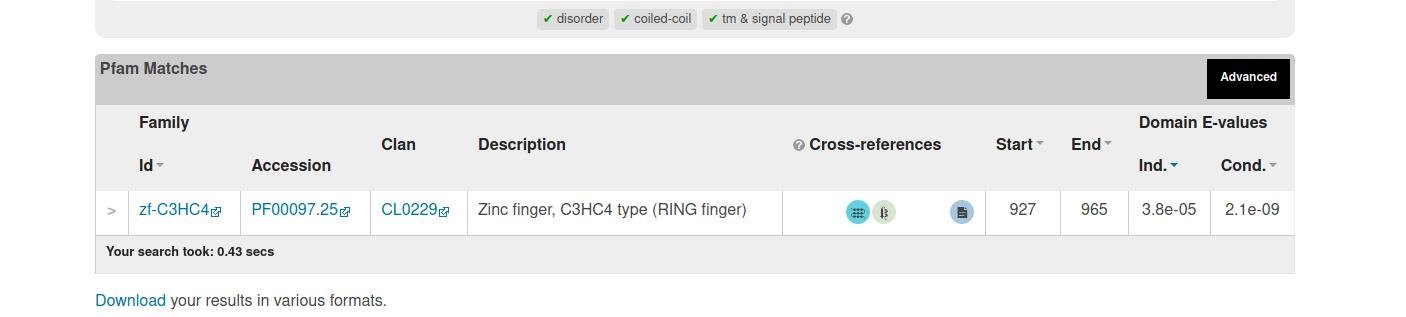
\includegraphics[scale=0.53]{1}  
 	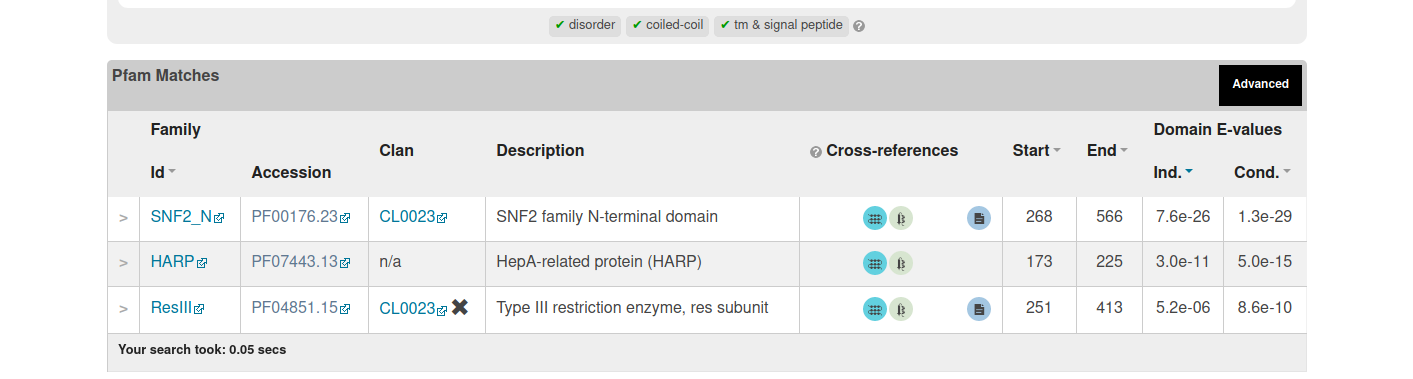
\includegraphics[scale=0.53]{2}
 	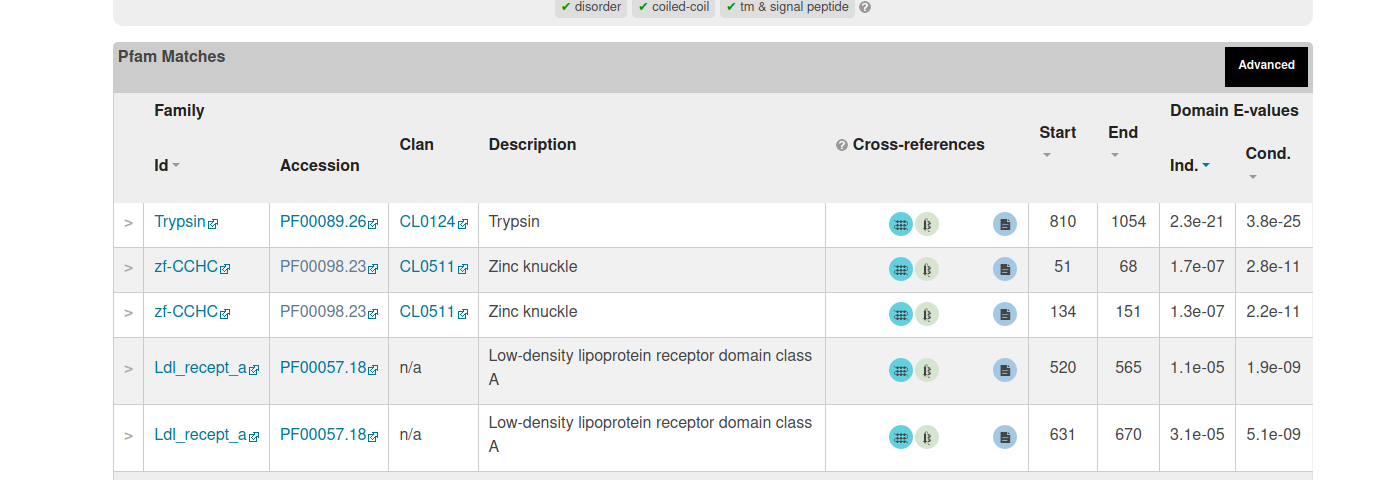
\includegraphics[scale=0.53]{3}
 	\caption{ HMMR }
 	\label{tree}
 \end{figure}
 
 
 
 
%\newpage 
\newpage 
\begin{thebibliography}{9}
	
	\bibitem{1}
	https://en.wikipedia.org/wiki/Tardigrade
	
	\bibitem{2}
	  McGinnis, S. and Madden, T. L. (2004). BLAST: at the core ofa powerful and diverse set of sequence analysis tools.Nucleic Acids Res, 32(Web Serverissue):W20--W25.
	
	\bibitem{3}
	Smith, T. F. and Waterman, M. S. (1981). Identification of commonmolecular subsequences.J Mol Biol, 147(1):195--197
	
	
	\bibitem{4}
	https://en.wikipedia.org/wiki/Sequence\_homology
	
	
 \bibitem{data}
 https://www.ncbi.nlm.nih.gov/Taxonomy/Browser/wwwtax.cgi?id=947166

\bibitem{augustus}
http://bioinf.uni-greifswald.de/augustus/


 \bibitem{blast}
 BLAST® Command Line Applications User Manual [Internet]. Bethesda (MD): National Center for Biotechnology Information (US); 2008-. Building a BLAST database with your (local) sequences. Available from: https://www.ncbi.nlm.nih.gov/books/NBK279688/
 
 \bibitem{WOlf}
 https://wolfpsort.hgc.jp/
 
 \bibitem{ptarget}
  Detecting Sequence Signals in Targeting Peptides Using Deep Learning
 José Juan Almagro Armenteros, Marco Salvatore, Ole Winther, Olof Emanuelsson, Gunnar von Heijne, Arne Elofsson, and Henrik Nielsen
 Life Science Alliance 2 (5), e201900429. doi:10.26508/lsa.201900429 
 
 \bibitem{HMM}
 S.C. Potter, A. Luciani, S.R. Eddy Y. Park, R. Lopez and R.D. Finn,
 Nucleic Acids Research (2018) Web Server Issue 46:W200-W204. 
 
 \bibitem{5}
  https://www.uniprot.org/uniprot/Q03468
  
   
  \bibitem{6}
 https://en.wikipedia.org/wiki/RING_finger_domain
 
  
 \bibitem{7}
 http://www.unige.ch/medecine/nouspikel/ubiquitin.html
 
 
\end{thebibliography}




\end{document}
